\documentclass[11pt,a4paper]{article}
\usepackage[T1]{fontenc}
\usepackage[utf8]{inputenc}
\usepackage{mathpazo}
\usepackage[margin=2.2cm]{geometry}
\usepackage{amsmath,amssymb}
\usepackage{enumitem}
\usepackage{xcolor}
\usepackage{titlesec}
\usepackage{booktabs,tabularx,longtable,array}
\usepackage[colorlinks=true,linkcolor=blue!50!black,urlcolor=blue!50!black]{hyperref}
\usepackage[capitalise,noabbrev]{cleveref}
\usepackage[most]{tcolorbox}
\usepackage{tikz}
\usepackage[edges]{forest}
\usetikzlibrary{arrows.meta,positioning,fit,calc,backgrounds}

\definecolor{navy}{HTML}{14213D}
\definecolor{blue}{HTML}{2E6F95}
\definecolor{orange}{HTML}{C96A1B}
\definecolor{okgreen}{HTML}{2E7D32}
\definecolor{skelamber}{HTML}{B7791F}
\definecolor{plangray}{HTML}{6B7280}
\titleformat{\section}{\Large\bfseries\color{navy}}{\thesection}{0.6em}{}
\titleformat{\subsection}{\large\bfseries\color{blue}}{\thesubsection}{0.5em}{}
\titleformat{\subsubsection}{\normalsize\bfseries\color{navy}}{\thesubsubsection}{0.5em}{}
\titlespacing*{\section}{0pt}{14pt}{6pt}
\titlespacing*{\subsection}{0pt}{10pt}{3pt}
\setlist{itemsep=2pt,topsep=3pt,leftmargin=1.4em}
\setlength{\parindent}{0pt}
\setlength{\parskip}{5pt}
\emergencystretch=3em

\newtcolorbox{newc}[1]{colback=green!4,colframe=green!40!black,fonttitle=\bfseries\small,
  title={New concept: #1},boxrule=0.5pt,arc=2pt,left=5pt,right=5pt,top=3pt,bottom=3pt}
\newtcolorbox{keybox}[1][]{colback=blue!5,colframe=blue!60!black,boxrule=0.6pt,arc=2pt,left=7pt,right=7pt,top=5pt,bottom=5pt,#1}
\newtcolorbox{filebox}[2]{colback=gray!3,colframe=navy!70,fonttitle=\bfseries\small,
  title={\texttt{#1}\hfill\mdseries #2},boxrule=0.5pt,arc=2pt,left=5pt,right=5pt,top=3pt,bottom=3pt,fontupper=\small}

\newcommand{\done}{\textcolor{okgreen}{\textbf{implemented}}}
\newcommand{\skel}{\textcolor{skelamber}{\textbf{skeleton}}}
\newcommand{\planned}{\textcolor{plangray}{\textbf{planned}}}
\newcommand{\chk}{\textit{(check)}}
\newcommand{\code}[1]{{\small\ttfamily\begingroup\def\_{\textunderscore\allowbreak}\def\/{/\allowbreak}#1\endgroup}}
\newcommand{\wt}[1]{\textcolor{blue!60!black}{\small[walkthrough~§#1]}}
\newcommand{\gdot}{\textcolor{okgreen}{$\bullet$}}
\newcommand{\sdot}{\textcolor{skelamber}{$\bullet$}}
\newcommand{\pdot}{\textcolor{plangray}{$\circ$}}

\hypersetup{pdftitle={The twin codebase: files, dependencies and call flow}}

\begin{document}

\begin{center}
{\LARGE\bfseries\color{navy} The twin codebase: files, dependencies and call flow}\\[6pt]
{\large\color{navy} A code-level map of \texttt{src/twin/} and the trust-weighting code}\\[8pt]
{\color{gray} Branch \code{twin}, commit \code{b6268b5} (25 Nov 2026, after WP 1.1 and WP 1.2) \quad·\quad written 26 Nov 2026}
\end{center}

\begin{keybox}[title={\textbf{What this document is}},fonttitle=\color{white}\bfseries,colbacktitle=blue!60!black]
The first document, \emph{The scene digital twin, from data to referee} (``the walkthrough''), explains \emph{what} the twin does and \emph{why}. This one is about the code: which file does what (\cref{sec:files}), who imports whom (\cref{sec:deps}), and which function calls which when the code runs (\cref{sec:flows}). Where a concept is explained in the walkthrough, a blue tag such as \wt{6.3} points to it; this document does not repeat it.

Markers: \gdot{} \done{} (code and tests exist); \sdot{} \skel{} (signatures exist, bodies raise \code{NotImplementedError}); \pdot{} \planned{} (not in the repo yet; the roadmap work package is named). \chk{} marks what I inferred but did not run. All paths are relative to the repo root.

\textbf{Changed since the walkthrough} (commit \code{f4f669e}): WP 1.1 made \code{TwinRenderer.render} work (0.09--0.10\,ms per frame on the lab PC, EGL) and fixed the 1-ulp asset mismatch; WP 1.2 added \code{src/rlinf\_modified/algorithms/trust.py}. The twin test subset is now 69 tests, plus 37 trust-weighting tests (\code{docs/thesis/progress.md}).
\end{keybox}

\tableofcontents
\newpage

%=====================================================================
\section{The repository, as far as the twin is concerned}\label{sec:tree}
%=====================================================================
The repo is large (the vendored training runtime alone has hundreds of files). \Cref{fig:tree} shows only what the twin and the trust weighting touch.

\begin{figure}[h]
\centering
\begin{forest}
  for tree={font=\ttfamily\footnotesize, grow'=0, folder, folder indent=8pt, s sep=1.2pt, inner ysep=1.2pt, edge={gray!70}}
[imagine-to-achieve/
  [src/
    [twin/ \textrm{\scriptsize the scene twin (package)}
      [\gdot{} transforms.py \textrm{\scriptsize rotations and $4\times4$ poses}]
      [\gdot{} robot.py \textrm{\scriptsize UR5 DH table, FK, MJCF generator}]
      [\gdot{} repo\_import.py \textrm{\scriptsize loads the repo's \texttt{eef\_pose\_adapter.py} by path}]
      [\gdot{} ik.py \textrm{\scriptsize Jacobian, closed-form IK, DLS, path tracking}]
      [\gdot{} actions.py \textrm{\scriptsize action checks, actions $\to$ EEF $\to$ joints}]
      [\gdot{} render.py \textrm{\scriptsize off-screen rendering (masks: \sdot)}]
      [\sdot{} cameras.py \textrm{\scriptsize intrinsics, camera records, projection}]
      [\sdot{} scene.py \textrm{\scriptsize laptop, physics parameters, scene (T3)}]
      [\sdot{} init\_fit.py \textrm{\scriptsize per-episode fit and cache (T5)}]
      [\sdot{} session.py \textrm{\scriptsize per-env twin session (kinematics-only works)}]
      [assets/ur5.xml \textrm{\scriptsize generated MJCF, committed}]
    ]
    [rlinf\_modified/algorithms/
      [\gdot{} trust.py \textrm{\scriptsize trust-weighted rewards and advantages (WP 1.2)}]
      [\gdot{} advantages.py \textrm{\scriptsize synthetic-engine advantages, optional weights}]
    ]
  ]
  [scripts/
    [\gdot{} make\_twin\_ur5\_mjcf.py \textrm{\scriptsize writes \texttt{assets/ur5.xml}}]
    [\gdot{} make\_twin\_fk\_reference.py \textrm{\scriptsize writes the FK test fixture}]
    [\gdot{} twin\_view.py \textrm{\scriptsize interactive MuJoCo viewer}]
  ]
  [tests/
    [conftest.py \textrm{\scriptsize sets \texttt{MUJOCO\_GL=egl} on Linux}]
    [test\_twin\_*.py \textrm{\scriptsize 9 files, 69 tests}]
    [test\_trust\_weighting.py \textrm{\scriptsize 37 tests}]
    [fixtures/twin\_fk\_reference\_ur5.json]
  ]
  [third\_party/rlinf\_runtime/rlinf/ \textrm{\scriptsize vendored runtime: \emph{read}, never edited}
    [envs/world\_model/eef\_pose\_adapter.py \textrm{\scriptsize conversions reused by the twin}]
    [envs/world\_model/world\_model\_ctrl\_world\_env.py \textrm{\scriptsize Ctrl-World env (hook points)}]
    [algorithms/cross\_rank\_grpo.py \textrm{\scriptsize production advantages}]
  ]
  [stage15\_plugin/ \textrm{\scriptsize the plugin pattern \texttt{twin\_plugin/} will copy}]
  [docs/thesis/ \textrm{\scriptsize roadmap, progress log, plan, guide, notes}]
  [CLAUDE.md \textrm{\scriptsize rules for Claude Code}]
]
\end{forest}
\caption{The part of the repository the twin lives in. Coloured dots: \gdot{} implemented, \sdot{} skeleton.}
\label{fig:tree}
\end{figure}

\textbf{Three things about the layout.}
\begin{itemize}
\item \textbf{\code{src/} layout.} \code{pyproject.toml} sets \code{package-dir = \{"" = "src"\}}, and pytest uses \code{pythonpath = ["src"]}. That is why the code writes \code{from twin.ik import ...}, not \code{from src.twin...}. Scripts in \code{scripts/} add \code{src/} to \code{sys.path} themselves.
\item \textbf{The vendored runtime is read, never edited.} The twin reuses three functions of \code{eef\_pose\_adapter.py} by loading that file directly (\cref{sec:repoimport}); integration will patch the runtime at run time from \code{twin\_plugin/}, not by editing it \wt{8.1}.
\item \textbf{Generated files are never hand-edited.} \code{assets/ur5.xml} and the FK fixture are written by scripts, and tests check that they match.
\end{itemize}

%=====================================================================
\section{The dependency graph}\label{sec:deps}
%=====================================================================
\Cref{fig:deps} shows which module imports which. An arrow $A\to B$ means ``$A$ imports from $B$'', labelled with what it imports. The modules are drawn in layers: every module only imports from layers below it, so there are no import cycles.

\begin{figure}[h]
\centering
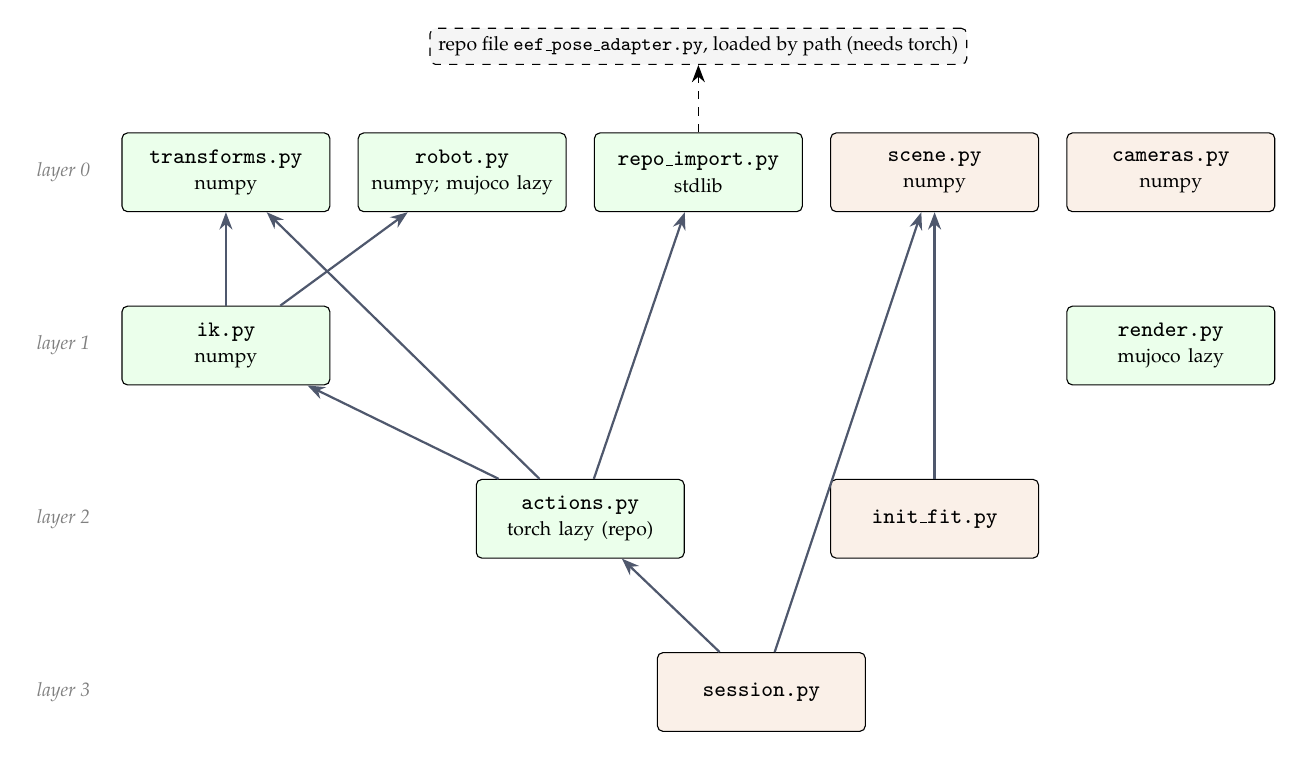
\begin{tikzpicture}[>={Stealth[length=2.2mm]},
  mod/.style={draw,rounded corners=2pt,font=\footnotesize,minimum height=10mm,text width=25mm,inner sep=2pt,align=center,fill=#1},
  mod/.default=white,
  ext/.style={draw,dashed,rounded corners=2pt,font=\scriptsize,inner sep=3pt,align=center,fill=gray!8},
  layer/.style={font=\scriptsize\itshape,text=gray,anchor=east},
  imp/.style={->,thick,navy!75}]
\node[layer] at (-0.4,0) {layer 0};
\node[layer] at (-0.4,-2.2) {layer 1};
\node[layer] at (-0.4,-4.4) {layer 2};
\node[layer] at (-0.4,-6.6) {layer 3};
% layer 0
\node[mod=green!8] (tr) at (1.2,0) {\texttt{transforms.py}\\ \scriptsize numpy};
\node[mod=green!8] (rb) at (4.2,0) {\texttt{robot.py}\\ \scriptsize numpy; mujoco lazy};
\node[mod=green!8] (ri) at (7.2,0) {\texttt{repo\_import.py}\\ \scriptsize stdlib};
\node[mod=orange!10] (sc) at (10.2,0) {\texttt{scene.py}\\ \scriptsize numpy};
\node[mod=orange!10] (cam) at (13.2,0) {\texttt{cameras.py}\\ \scriptsize numpy};
\node[mod=green!8] (rd) at (13.2,-2.2) {\texttt{render.py}\\ \scriptsize mujoco lazy};
% higher layers
\node[mod=green!8] (ik) at (1.2,-2.2) {\texttt{ik.py}\\ \scriptsize numpy};
\node[mod=green!8] (ac) at (5.7,-4.4) {\texttt{actions.py}\\ \scriptsize torch lazy (repo)};
\node[mod=orange!10] (ifit) at (10.2,-4.4) {\texttt{init\_fit.py}};
\node[mod=orange!10] (se) at (8.0,-6.6) {\texttt{session.py}};
% external
\node[ext] (eef) at (7.2,1.6) {repo file \texttt{eef\_pose\_adapter.py}, loaded by path (needs torch)};
% edges (importer -> imported)
\draw[imp] (ik) -- (tr);
\draw[imp] (ik) -- (rb);
\draw[imp] (ac) -- (ik);
\draw[imp] (ac) -- (ri);
\draw[imp] (ac) -- (tr);
\draw[imp] (se) -- (ac);
\draw[imp] (se) -- (sc);
\draw[imp] (ifit) -- (sc);
\draw[->,dashed] (ri) -- (eef);
\end{tikzpicture}
\caption{Import graph of \code{src/twin/}. An arrow $A\to B$ means ``$A$ imports from $B$''. Green: implemented; orange: skeleton. \code{render.py} and \code{cameras.py} import nothing from the package yet. The names imported along each arrow are in \cref{tab:imports}.}
\label{fig:deps}
\end{figure}

\begin{table}[h]
\centering\small
\begin{tabularx}{\linewidth}{@{}>{\raggedright\arraybackslash}p{3.0cm}>{\raggedright\arraybackslash}p{2.6cm}X@{}}
\toprule
\textbf{Module} & \textbf{imports from} & \textbf{names}\\
\midrule
\code{ik.py} & \code{robot} & \code{UR5\_DH}, \code{TCP\_OFFSET}, \code{JOINT\_LIMITS}, \code{dh\_transform}, \code{fk}\\
 & \code{transforms} & \code{so3\_log}, \code{make\_T}, \code{invert\_T}, \code{geodesic\_angle}\\
\code{actions.py} & \code{ik} & \code{track\_path}, \code{IKConfig}, \code{DEFAULT\_IK}, \code{PathIKResult}, \code{UR5\_MAX\_JOINT\_SPEED}\\
 & \code{repo\_import} & \code{load\_eef\_pose\_adapter}\\
 & \code{transforms} & \code{rotvec\_to\_matrix}, \code{make\_T}, \code{invert\_T}, \code{geodesic\_angle}\\
\code{init\_fit.py} & \code{scene} & \code{SceneState}\\
\code{session.py} & \code{actions} & \code{ActionsToJoints}, \code{JointChunk}\\
 & \code{scene} & \code{LaptopScene}, \code{SceneState}, \code{ChunkRollout}\\
\midrule
\code{scripts/make\_twin\_ur5\_mjcf.py} & \code{robot} & \code{ur5\_mjcf\_xml}, \code{UR5\_ASSET\_PATH}\\
\code{scripts/make\_twin\_fk\_reference.py} & \code{robot}, \code{repo\_import} & \code{fk}, \code{TCP\_OFFSET}, \code{JOINT\_LIMITS}; \code{load\_eef\_pose\_adapter}\\
\code{scripts/twin\_view.py} & \code{session}, \code{actions}, \code{robot}, \code{transforms} & inside functions: \code{TwinSession}, \code{ActionsToJoints}, \code{identity\_actions}, \code{fk}, \code{load\_ur5\_model}, \code{so3\_log}\\
\bottomrule
\end{tabularx}
\caption{What each import arrow carries, and the scripts that use the package.}
\label{tab:imports}
\end{table}

\textbf{How to read it.}
\begin{itemize}
\item \textbf{Layer 0 has no internal dependencies.} \code{transforms.py} and \code{robot.py} need only numpy; \code{repo\_import.py} only the standard library. \code{scene.py} and \code{cameras.py} are skeletons that so far only define data classes.
\item \textbf{\code{ik.py} depends on the robot model}, because IK is ``FK run backwards'' and must use exactly the same DH table.
\item \textbf{\code{actions.py} is the hub of T2.} It is the only module that touches the repo's conversion code, and it hands its result to \code{ik.py}.
\item \textbf{\code{session.py} is the top}: it combines the kinematics (\code{actions.py}) and the physics (\code{scene.py}) for one environment \wt{6.8}.
\item \textbf{Heavy libraries are imported lazily.} \code{torch} is imported inside \code{actions\_to\_eef\_targets} (through the repo file); \code{mujoco} inside \code{load\_ur5\_model} and \code{TwinRenderer}. So \code{import twin.ik} works on a machine without torch or MuJoCo, and the numpy-only tests run anywhere.
\end{itemize}

\begin{newc}{lazy import}
An \code{import} written inside a function instead of at the top of the file. It runs only when the function is first called. Here it keeps optional, heavy dependencies (torch, MuJoCo, an OpenGL context) out of modules that do not always need them.
\end{newc}

\subsection{The trust-weighting code}
The second piece of thesis code lives elsewhere, in \code{src/rlinf\_modified/algorithms/}, because it is about the RL update, not the scene.

\begin{figure}[h]
\centering
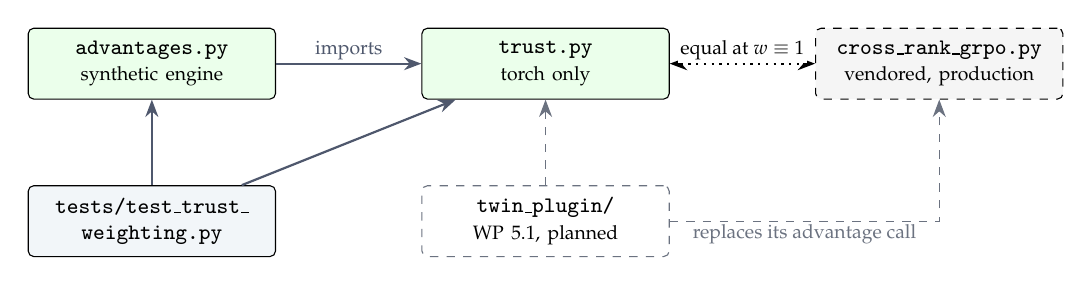
\begin{tikzpicture}[>={Stealth[length=2.2mm]},
  mod/.style={draw,rounded corners=2pt,font=\footnotesize,minimum height=9mm,text width=30mm,inner sep=2pt,align=center,fill=#1},
  lab/.style={font=\scriptsize,fill=white,inner sep=1pt,align=center}]
\node[mod=green!8] (tw) at (0,0) {\texttt{trust.py}\\ \scriptsize torch only};
\node[mod=green!8] (adv) at (-5.0,0) {\texttt{advantages.py}\\ \scriptsize synthetic engine};
\node[mod=blue!6] (t) at (-5.0,-2.0) {\texttt{tests/test\_trust\_}\\ \texttt{weighting.py}};
\node[mod=white,dashed,draw=plangray] (pl) at (0,-2.0) {\texttt{twin\_plugin/}\\ \scriptsize WP 5.1, planned};
\node[mod=gray!8,dashed] (cr) at (5.0,0) {\texttt{cross\_rank\_grpo.py}\\ \scriptsize vendored, production};
\draw[->,thick,navy!75] (adv) -- node[lab,above]{imports} (tw);
\draw[->,thick,navy!75] (t) -- (adv); \draw[->,thick,navy!75] (t) -- (tw);
\draw[->,dashed,plangray] (pl) -- (tw);
\draw[->,dashed,plangray] (pl) -| node[lab,pos=0.25,below]{replaces its advantage call} (cr);
\draw[<->,dotted,thick] (tw) -- node[lab,above]{equal at $w\equiv1$} (cr);
\end{tikzpicture}
\caption{Trust weighting. \code{trust.py} stands alone; \code{advantages.py} calls it when \code{weights} is given; the plugin (planned) will call it in production, where the tests already show it equals the vendored function bit for bit at full trust.}
\label{fig:trustdeps}
\end{figure}

%=====================================================================
\section{File by file}\label{sec:files}
%=====================================================================
Each box lists the role of the file, its public names, and its status. Private helpers (leading underscore) are mentioned only when they matter for understanding.

\subsection{Layer 0}

\begin{filebox}{src/twin/transforms.py}{implemented · 120 lines}
\textbf{Role:} the rotation and pose maths every other module uses \wt{5}. numpy only, batched over leading axes.
\begin{center}
\begin{tabularx}{\linewidth}{@{}>{\raggedright\arraybackslash}p{5.0cm}X@{}}
\toprule
\textbf{Name} & \textbf{What it does}\\
\midrule
\code{skew(v)} & $3\times3$ matrix $[v]_\times$ with $[v]_\times u = v\times u$\\
\code{rotvec\_to\_matrix(r)} & axis-angle vector to rotation matrix (Rodrigues' formula)\\
\code{so3\_log(R)} & rotation matrix to axis-angle vector; accurate up to $\pi-10^{-9}$\\
\code{geodesic\_angle(Ra, Rb)} & angle of $R_a^\top R_b$, via \code{atan2} (accurate near $0$ and $\pi$)\\
\code{make\_T(R, p), invert\_T(T)} & build a $4\times4$ pose; invert it using $R^\top$\\
\bottomrule
\end{tabularx}
\end{center}
\end{filebox}

\begin{filebox}{src/twin/robot.py}{implemented · 178 lines}
\textbf{Role:} the UR5 model, numerically and for MuJoCo \wt{6.1}.
\begin{center}
\begin{tabularx}{\linewidth}{@{}>{\raggedright\arraybackslash}p{5.0cm}X@{}}
\toprule
\textbf{Name} & \textbf{What it does}\\
\midrule
\code{UR5\_DH, TCP\_OFFSET} & the six $(a,d,\alpha)$ rows read from the repo; tool offset $(0,0,0.18)$\,m\\
\code{JOINT\_LIMITS, JOINT\_NAMES, LINK\_NAMES} & $\pm2\pi$ per joint; names used in the MJCF\\
\code{dh\_transform(a, d, alpha, theta)} & one link transform $R_z(\theta)T_z(d)T_x(a)R_x(\alpha)$\\
\code{fk(q, tcp=True)} & forward kinematics, $(\ldots,6)\to(\ldots,4,4)$\\
\code{ur5\_mjcf\_xml()} & builds the MJCF text from \code{UR5\_DH}; no MuJoCo import. Uses \code{\_rx\_quat} (exact quarter turns with \code{sqrt(0.5)}, WP 1.1), \code{\_num}, \code{\_vec} for formatting\\
\code{UR5\_ASSET\_PATH} & \code{src/twin/assets/ur5.xml}\\
\code{load\_ur5\_model()} & \code{mujoco.MjModel.from\_xml\_string(ur5\_mjcf\_xml())} (lazy import)\\
\bottomrule
\end{tabularx}
\end{center}
The MJCF places every body frame on its own joint axis (hinge about $+z$, \code{qpos} $=q$), with sites \code{flange} and \code{tcp}. Geoms are visual-only capsules (\code{contype="0"}), so the arm has no collisions yet.
\end{filebox}

\begin{filebox}{src/twin/repo\_import.py}{implemented · 37 lines}\label{sec:repoimport}
\textbf{Role:} gives the twin the repo's own conversion functions, so it cannot drift from production.

\code{load\_eef\_pose\_adapter()} loads \code{third\_party/.../envs/world\_model/eef\_pose\_adapter.py} \emph{by file path} with \code{importlib}, registers it in \code{sys.modules} under a private name, and caches it (\code{functools.cache}). Loading by path avoids \code{import rlinf...}, which would execute the runtime's package \code{\_\_init\_\_} and pull in Ray and the whole training stack. \code{EEF\_POSE\_ADAPTER\_PATH} is the file's location.
\end{filebox}

\begin{filebox}{src/twin/scene.py}{skeleton · 130 lines}
\textbf{Role:} the physical scene of T3 \wt{6.4}. Data classes exist; \code{LaptopScene}'s methods raise \code{NotImplementedError}.
\begin{center}
\begin{tabularx}{\linewidth}{@{}>{\raggedright\arraybackslash}p{5.0cm}X@{}}
\toprule
\textbf{Name} & \textbf{What it is}\\
\midrule
\code{PHYSICS\_TIMESTEP, SUBSTEPS\_PER\_FRAME} & $1/480$\,s; 16 physics steps per 30\,Hz frame\\
\code{LaptopGeometry, DEFAULT\_GEOMETRY} & box sizes, hinge offset, maximum opening (placeholders)\\
\code{PhysicsParams, DEFAULT\_PARAMS} & one $\psi$: hinge friction, damping, masses, friction coefficients, contact softness, lag\\
\code{SceneState} & $x=(p_x,p_y,\text{yaw},\vartheta)$ plus joints and gripper\\
\code{GripperModel.opening(g)} & \gdot{} absolute gripper value $\to$ finger opening (linear, clipped; implemented)\\
\code{ChunkRollout} & per-frame record of one chunk (lid angle, contacts, penetration)\\
\code{LaptopScene: mjcf\_xml, reset, step\_chunk, get\_state} & \sdot{} the scene itself (WP 2.3)\\
\bottomrule
\end{tabularx}
\end{center}
\end{filebox}

\begin{filebox}{src/twin/cameras.py}{skeleton · 70 lines}
\textbf{Role:} camera parameters \wt{6.5}. \code{PHYSICAL\_CAMERAS} (\code{d405\_0\_rgb}, \code{d405\_1\_rgb}, \code{d435\_rgb}), \code{DATASET\_IMAGE\_SIZE} $(480,640)$, \code{LOOP\_IMAGE\_SIZE} $(192,320)$; \code{CameraIntrinsics} with \code{K} and \code{resized(h, w)}; \code{Camera} (name, intrinsics, pose, wrist flag); \code{project(K, T\_WC, p\_W)} (pinhole projection, implemented). Building MJCF cameras from these is WP 3.1.
\end{filebox}

\subsection{Layers 1 to 3}

\begin{filebox}{src/twin/ik.py}{implemented · 358 lines}
\textbf{Role:} joint angles for end-effector poses \wt{6.3}. numpy only.
\begin{center}
\begin{tabularx}{\linewidth}{@{}>{\raggedright\arraybackslash}p{5.0cm}X@{}}
\toprule
\textbf{Name} & \textbf{What it does}\\
\midrule
\code{joint\_frames(q)} & the 7 frames $T_{B,i}$ along the arm, $(7,4,4)$\\
\code{jacobian(q)} & geometric Jacobian $(6,6)$ at the TCP, from \code{joint\_frames}\\
\code{branch\_of(q)} & which of the 8 UR5 solution families (shoulder, elbow, wrist) $q$ belongs to\\
\code{ik\_analytic(T\_BE)} & closed-form IK: all solutions, up to 8\\
\code{nearest\_equivalent, initial\_configuration} & pick the solution closest to a reference pose (when only an EEF pose is known)\\
\code{IKConfig, DEFAULT\_IK} & tolerances ($10^{-6}$), damping settings, max step, joint limits\\
\code{pose\_error(T\_target, T)} & 6-D error: position difference and \code{so3\_log} of the rotation difference\\
\code{ik\_dls(T\_target, q\_seed) $\to$ IKResult} & damped least squares from a warm start\\
\code{track\_path(T\_targets, q\_start, dt) $\to$ PathIKResult} & \code{ik\_dls} frame by frame, each seeded with the previous solution, plus feasibility flags\\
\code{UR5\_MAX\_JOINT\_SPEED} & $\pi$\,rad/s per joint (180\,deg/s) \chk\\
\bottomrule
\end{tabularx}
\end{center}
\end{filebox}

\begin{filebox}{src/twin/render.py}{render implemented, masks skeleton · 51 lines}
\textbf{Role:} images of the twin \wt{6.5}. \code{TwinRenderer(model, height=192, width=320)} keeps one \code{mujoco.Renderer} (the OpenGL context is expensive, so it is reused). \code{render(data, camera)} checks that the camera exists (\code{mj\_name2id}, else \code{KeyError}), then \code{update\_scene} and \code{render}, and returns a new \code{uint8} array $(H,W,3)$. It never calls \code{mj\_forward} and never changes \code{data}: the caller keeps the state up to date. \code{render\_masks} is T4 (WP 3.1). Usable as a context manager (\code{with TwinRenderer(...) as r:}).
\end{filebox}

\begin{filebox}{src/twin/actions.py}{implemented · 360 lines}
\textbf{Role:} one policy chunk to 64 joint targets, exactly as production converts it \wt{6.2}.
\begin{center}
\begin{tabularx}{\linewidth}{@{}>{\raggedright\arraybackslash}p{5.0cm}X@{}}
\toprule
\textbf{Name} & \textbf{What it does}\\
\midrule
\code{ACTION\_DIM, identity\_actions(n)} & 10; a chunk that does not move\\
\code{ActionCheckConfig, check\_actions(a) $\to$ ActionReport} & hard errors (shape, NaN, degenerate rot6d) and warnings (large steps, gripper range)\\
\code{AdapterConfig, PRODUCTION\_ADAPTER} & resolved production settings (gains, frame, 15/30\,Hz, gripper clip)\\
\code{actions\_to\_eef\_targets(state, a) $\to$ EEFTargets} & the repo conversion in float32: chain, clip, resample, Ctrl-World alignment\\
\code{eef\_state\_to\_T(states)} & 7-D EEF state (axis-angle) to $4\times4$ poses\\
\code{ActionsToJoints(T\_WB).step\_chunk(state, a, q) $\to$ JointChunk} & checks + EEF targets + $T_{WB}^{-1}$ + \code{track\_path}\\
\bottomrule
\end{tabularx}
\end{center}
\end{filebox}

\begin{filebox}{src/twin/init\_fit.py}{skeleton · 35 lines}
\textbf{Role:} the per-episode scene fit of Step~2 \wt{6.6}. \code{EpisodeFit} (episode id, best and near-optimal \code{SceneState}s, IoU per view, $q_0$); \code{SCENE\_CACHE\_DIR} $=$ \code{scene\_cache/}; \code{fit\_episode} and \code{load\_cached\_fit} raise \code{NotImplementedError} (WP 3.2).
\end{filebox}

\begin{filebox}{src/twin/session.py}{kinematics implemented, physics skeleton · 73 lines}
\textbf{Role:} the twin of one environment through an episode \wt{6.8}. \code{TwinSession(actions\_to\_joints, scene=None)} with \code{reset(eef\_state, q0, scene\_state=None)}, \code{step\_chunk(actions)} $\to$ \code{ChunkResult} (joints, rollout, renders) and \code{reachability\_summary()}. It carries two pieces of state between chunks: the open-loop EEF state (\code{next\_state}, as Ctrl-World does) and the last joint vector (the IK seed for the next chunk).
\end{filebox}

\subsection{Trust weighting}

\begin{filebox}{src/rlinf\_modified/algorithms/trust.py}{implemented · 207 lines}
\textbf{Role:} proposal Step~8.2: imputed rewards (eq.~20) inside the group-normalised suffix advantages (eq.~4), with both scale options of decision D1 \wt{7}.
\begin{center}
\begin{tabularx}{\linewidth}{@{}>{\raggedright\arraybackslash}p{5.2cm}X@{}}
\toprule
\textbf{Name} & \textbf{What it does}\\
\midrule
\code{group\_members(group\_index)} & column indices of every group, $[\text{groups},G]$; groups need not be contiguous (production groups span ranks)\\
\code{suffix\_returns(r, dones, gamma)} & $R_{ik}=\sum_{j\ge k}\gamma^{j-k}r_{ij}$, cut at done boundaries; same operations as the old function\\
\code{trust\_weighted\_rewards(r, w, group\_index)} & eq.~(20) only: $\hat r$\\
\code{trust\_weighted\_suffix\_advantages(...) $\to$ (A, TrustStats)} & the full computation; \code{std\_source} $\in\{$\code{"weighted"} (A, default), \code{"unweighted"} (B)$\}$\\
\code{TrustStats} & share of $w<1$, mean $w$, std ratio per group and chunk, max $|A|$\\
\code{\_impute, \_normalise, \_check\_weights} & building blocks; tests call \code{\_impute} directly for $w=0$ (P14(c)), which the public functions reject\\
\bottomrule
\end{tabularx}
\end{center}
\end{filebox}

\begin{filebox}{src/rlinf\_modified/algorithms/advantages.py}{implemented · 84 lines}
\textbf{Role:} the synthetic engine's advantage function \code{grpo\_action\_suffix\_advantages}, now with optional \code{weights} and \code{std\_source}. With \code{weights=None} the original lines run unchanged (tested against a frozen copy); otherwise it builds a contiguous group index and calls \code{trust\_weighted\_suffix\_advantages}.
\end{filebox}

\subsection{Scripts and tests}

\begin{center}\small
\begin{tabularx}{\linewidth}{@{}>{\raggedright\arraybackslash}p{5.0cm}X@{}}
\toprule
\textbf{Script} & \textbf{What it does}\\
\midrule
\code{make\_twin\_ur5\_mjcf.py} & writes \code{ur5\_mjcf\_xml()} to \code{assets/ur5.xml} with \code{\textbackslash n} line endings (same bytes on Windows and Linux)\\
\code{make\_twin\_fk\_reference.py} & 1000 random joint vectors through the repo's \code{ur5\_joint\_actions\_to\_eef\_states} in float64 $\to$ \code{tests/fixtures/twin\_fk\_reference\_ur5.json}, with source hash and commit\\
\code{twin\_view.py} & viewer: \code{--model ur5}, \code{--replay q.json/.npz}, \code{--demo-chunk [--chunks N]}, \code{--loop}\\
\bottomrule
\end{tabularx}
\end{center}

\begin{center}\small
\begin{tabularx}{\linewidth}{@{}>{\raggedright\arraybackslash}p{5.0cm}>{\raggedright\arraybackslash}p{3.0cm}X@{}}
\toprule
\textbf{Test file} & \textbf{Covers} & \textbf{Main checks}\\
\midrule
\code{test\_twin\_fk.py} & \code{robot}, \code{transforms} & numpy FK = repo FK (fixture); rotation helpers\\
\code{test\_twin\_mujoco\_fk.py} & \code{robot} (MJCF) & MuJoCo \code{tcp} site = repo FK; asset file = generator output; exact quarter turns\\
\code{test\_twin\_ik.py} & \code{ik} & Jacobian vs finite differences and \code{mj\_jacSite}; FK(IK); singularities\\
\code{test\_twin\_actions.py} & \code{actions} & bit-equality with the production conversion; action checks\\
\code{test\_twin\_action\_to\_joints.py} & \code{actions}, \code{ik} & five chained chunks, offset $T_{WB}$\\
\code{test\_twin\_skeleton.py} & \code{scene}, \code{cameras}, \code{session} & gripper map, projection, scene stub raises, kinematics-only session\\
\code{test\_twin\_render.py} & \code{render} & shape, determinism, unknown camera; timing in \code{\_\_main\_\_}\\
\code{test\_twin\_view\_script.py} & \code{twin\_view.py} & argument parsing, file loading, demo chunk (no window)\\
\code{test\_trust\_weighting.py} & \code{trust}, \code{advantages} & $w=1$ parity (both functions), P14, Lemma~1, D1\\
\bottomrule
\end{tabularx}
\end{center}
Run them with \code{python -m pytest tests/test\_twin\_*.py tests/test\_trust\_weighting.py -q}. On Linux, \code{tests/conftest.py} sets \code{MUJOCO\_GL=egl} before MuJoCo is imported (an explicit value wins); render tests skip, not fail, if no OpenGL context can be created.

%=====================================================================
\section{Call flows}\label{sec:flows}
%=====================================================================
This section follows what happens when the code runs. Boxes are functions; an arrow means ``calls''; grey text gives the data passed, with shapes.

\subsection{One chunk through the twin (today: kinematics only)}\label{sec:chunkflow}
This is the path every chunk will take in training. It is what \code{TwinSession.step\_chunk} runs today; once T3 exists, the last call (dashed) adds the physics.

\begin{figure}[p]
\centering
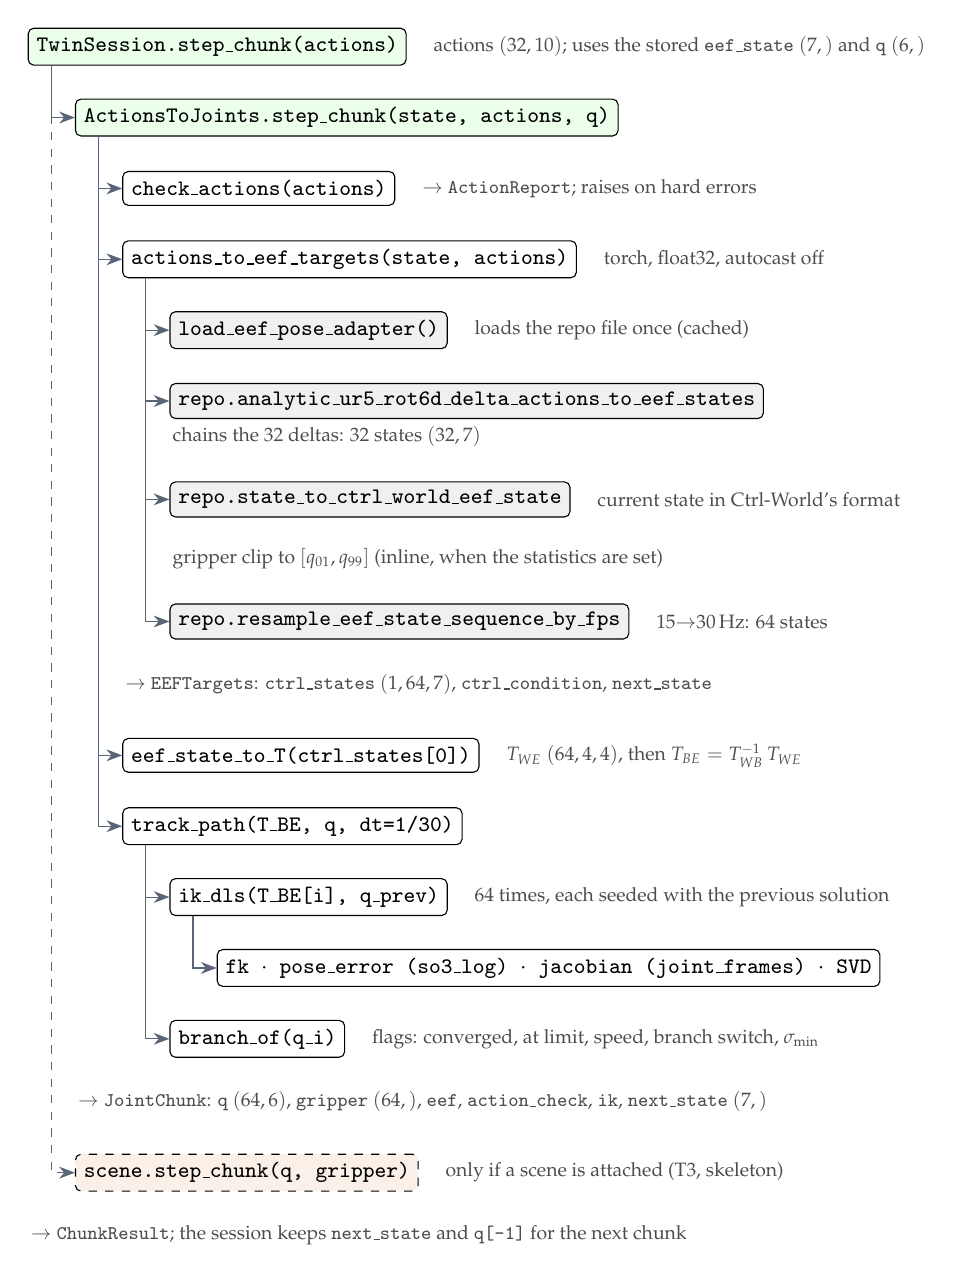
\begin{tikzpicture}[>={Stealth[length=2mm]},
  fn/.style={draw,rounded corners=2pt,font=\footnotesize\ttfamily,inner sep=3pt,anchor=west,fill=#1},
  fn/.default=white,
  dat/.style={font=\scriptsize,text=gray!60!black,anchor=west,align=left,inner sep=1pt},
  call/.style={->,draw=navy!70}]
\node[fn=green!8] (ss) at (0,0) {TwinSession.step\_chunk(actions)};
\node[dat,right=3mm of ss] {actions $(32,10)$; uses the stored \texttt{eef\_state} $(7,)$ and \texttt{q} $(6,)$};
\node[fn=green!8] (a2j) at (0.6,-0.9) {ActionsToJoints.step\_chunk(state, actions, q)};
\node[fn] (chk) at (1.2,-1.8) {check\_actions(actions)};
\node[dat,right=3mm of chk] {$\to$ \texttt{ActionReport}; raises on hard errors};
\node[fn] (e2t) at (1.2,-2.7) {actions\_to\_eef\_targets(state, actions)};
\node[dat,right=3mm of e2t] {torch, float32, autocast off};
\node[fn=gray!12] (ld) at (1.8,-3.6) {load\_eef\_pose\_adapter()};
\node[dat,right=3mm of ld] {loads the repo file once (cached)};
\node[fn=gray!12] (r1) at (1.8,-4.5) {repo.analytic\_ur5\_rot6d\_delta\_actions\_to\_eef\_states};
\node[dat,below=0.5mm of r1.south west,anchor=north west] {chains the 32 deltas: 32 states $(32,7)$};
\node[fn=gray!12] (r2) at (1.8,-5.75) {repo.state\_to\_ctrl\_world\_eef\_state};
\node[dat,right=3mm of r2] {current state in Ctrl-World's format};
\node[dat] (clip) at (1.8,-6.5) {gripper clip to $[q_{01},q_{99}]$ (inline, when the statistics are set)};
\node[fn=gray!12] (r3) at (1.8,-7.3) {repo.resample\_eef\_state\_sequence\_by\_fps};
\node[dat,right=3mm of r3] {15$\to$30\,Hz: 64 states};
\node[dat] at (1.2,-8.1) {$\to$ \texttt{EEFTargets}: \texttt{ctrl\_states} $(1,64,7)$, \texttt{ctrl\_condition}, \texttt{next\_state}};
\node[fn] (st) at (1.2,-9.0) {eef\_state\_to\_T(ctrl\_states[0])};
\node[dat,right=3mm of st] {$T_{WE}$ $(64,4,4)$, then $T_{BE}=T_{WB}^{-1}\,T_{WE}$};
\node[fn] (tp) at (1.2,-9.9) {track\_path(T\_BE, q, dt=1/30)};
\node[fn] (dls) at (1.8,-10.8) {ik\_dls(T\_BE[i], q\_prev)};
\node[dat,right=3mm of dls] {64 times, each seeded with the previous solution};
\node[fn] (inner) at (2.4,-11.7) {fk $\cdot$ pose\_error (so3\_log) $\cdot$ jacobian (joint\_frames) $\cdot$ SVD};
\node[fn] (br) at (1.8,-12.6) {branch\_of(q\_i)};
\node[dat,right=3mm of br] {flags: converged, at limit, speed, branch switch, $\sigma_{\min}$};
\node[dat] at (0.6,-13.4) {$\to$ \texttt{JointChunk}: \texttt{q} $(64,6)$, \texttt{gripper} $(64,)$, \texttt{eef}, \texttt{action\_check}, \texttt{ik}, \texttt{next\_state} $(7,)$};
\node[fn=orange!10,dashed] (sc) at (0.6,-14.3) {scene.step\_chunk(q, gripper)};
\node[dat,right=3mm of sc] {only if a scene is attached (T3, skeleton)};
\node[dat] at (0,-15.1) {$\to$ \texttt{ChunkResult}; the session keeps \texttt{next\_state} and \texttt{q[-1]} for the next chunk};
\foreach \p/\c in {ss/a2j,a2j/chk,a2j/e2t,e2t/ld,e2t/r1,e2t/r2,e2t/r3,a2j/st,a2j/tp,tp/dls,dls/inner,tp/br}{
  \draw[call] ([xshift=3mm]\p.south west) |- (\c.west);
}
\draw[call,dashed] ([xshift=3mm]ss.south west) |- (sc.west);
\end{tikzpicture}
\caption{Call tree of one chunk. Grey boxes: the repo's own functions, loaded by path; white: twin code; dashed: T3, not implemented yet.}
\label{fig:chunkflow}
\end{figure}

\textbf{Two design points visible in the call tree.}
\begin{itemize}
\item \textbf{The repo functions are called, not re-implemented.} \code{actions\_to\_eef\_targets} goes through the same three functions as \code{CtrlWorldEnv.\_convert\_via\_analytic\_ur5\_rot6d} in production, in float32, so the twin's 64 targets equal Ctrl-World's conditioning bit for bit.
\item \textbf{The two pieces of state are chained.} The EEF state for the next chunk is the repo's \code{next\_state} (open loop, like Ctrl-World); the IK seed for the next chunk is the last solved joint vector. So the arm follows exactly the commanded path; if it cannot, the IK flags say so.
\end{itemize}

\subsection{Model generation, rendering and the viewer}\label{sec:renderflow}

\begin{figure}[h]
\centering
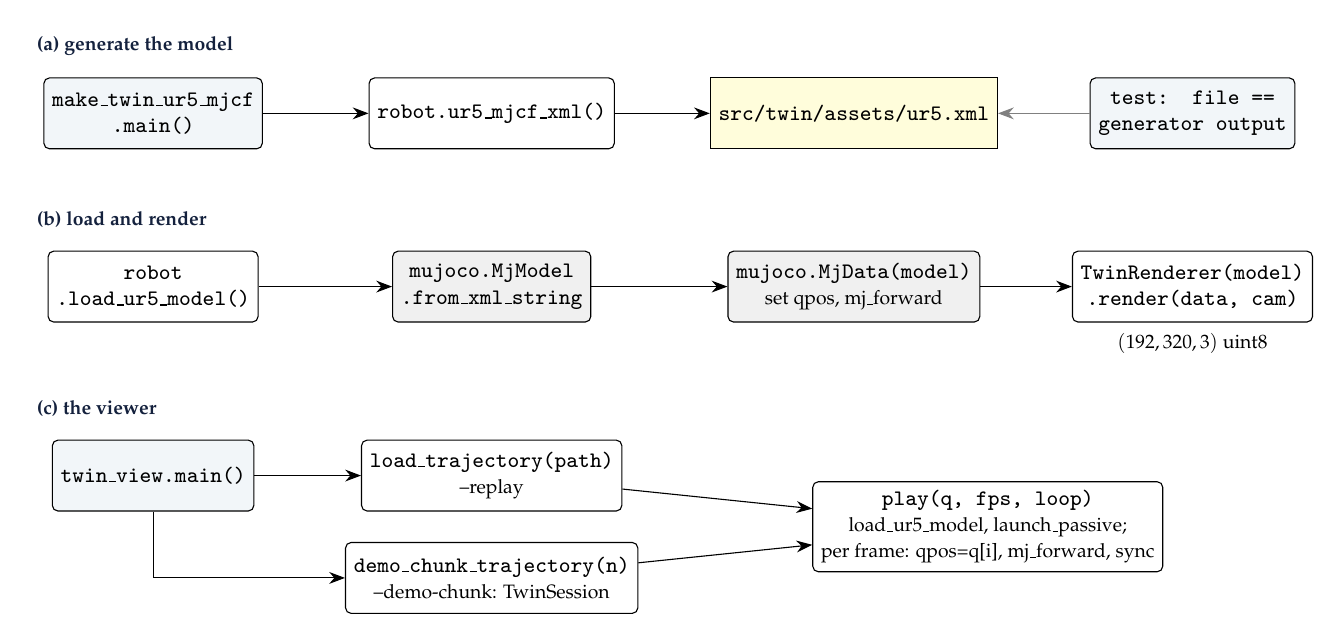
\begin{tikzpicture}[>={Stealth[length=2mm]},
  fn/.style={draw,rounded corners=2pt,font=\footnotesize\ttfamily,inner sep=3pt,align=center,fill=#1,minimum height=9mm},
  fn/.default=white,
  file/.style={draw,font=\footnotesize\ttfamily,fill=yellow!14,inner sep=3pt,minimum height=9mm,align=center},
  lab/.style={font=\scriptsize,fill=white,inner sep=1pt,align=center},
  row/.style={font=\scriptsize\bfseries,text=navy,anchor=west}]
\node[row] at (-1.6,0.85) {(a) generate the model};
\node[fn=blue!6] (mk) at (0,0) {make\_twin\_ur5\_mjcf\\ .main()};
\node[fn] (gen) at (4.3,0) {robot.ur5\_mjcf\_xml()};
\node[file] (xml) at (8.9,0) {src/twin/assets/ur5.xml};
\node[fn=blue!6] (tst) at (13.2,0) {test: file ==\\ generator output};
\draw[->] (mk) -- (gen); \draw[->] (gen) -- (xml); \draw[->,gray] (tst) -- (xml);
\node[row] at (-1.6,-1.35) {(b) load and render};
\node[fn] (load) at (0,-2.2) {robot\\ .load\_ur5\_model()};
\node[fn=gray!12] (mod) at (4.3,-2.2) {mujoco.MjModel\\ .from\_xml\_string};
\node[fn=gray!12] (dat) at (8.9,-2.2) {mujoco.MjData(model)\\ \rmfamily\scriptsize set qpos, mj\_forward};
\node[fn] (rr) at (13.2,-2.2) {TwinRenderer(model)\\ .render(data, cam)};
\draw[->] (load) -- (mod); \draw[->] (mod) -- (dat); \draw[->] (dat) -- (rr);
\node[lab,below=1mm of rr] {$(192,320,3)$ uint8};
\node[row] at (-1.6,-3.75) {(c) the viewer};
\node[fn=blue!6] (vm) at (0,-4.6) {twin\_view.main()};
\node[fn] (lt) at (4.3,-4.6) {load\_trajectory(path)\\ \rmfamily\scriptsize --replay};
\node[fn] (dc) at (4.3,-5.9) {demo\_chunk\_trajectory(n)\\ \rmfamily\scriptsize --demo-chunk: TwinSession};
\node[fn] (pl) at (10.6,-5.25) {play(q, fps, loop)\\ \rmfamily\scriptsize load\_ur5\_model, launch\_passive;\\ \rmfamily\scriptsize per frame: qpos=q[i], mj\_forward, sync};
\draw[->] (vm) -- (lt); \draw[->] (vm) |- (dc);
\draw[->] (lt) -- (pl); \draw[->] (dc) -- (pl);
\end{tikzpicture}
\caption{(a) The robot model is generated and checked. (b) Loading and rendering: the renderer reads \code{data} and never changes it. (c) The viewer plays a joint path, from a file or from synthetic chunks run through the twin (\cref{fig:chunkflow}).}
\label{fig:renderflow}
\end{figure}

\begin{newc}{passive viewer}
\code{mujoco.viewer.launch\_passive(model, data)} opens a window that \emph{shows} \code{data} but does not step the simulation itself. The script sets \code{qpos} to the next frame of the path, calls \code{mj\_forward} (pose update, no physics), and \code{viewer.sync()} redraws. It is a kinematic replay, which is what you want for checking IK paths.
\end{newc}

\subsection{Trust-weighted advantages}\label{sec:trustflow}

\begin{figure}[h]
\centering
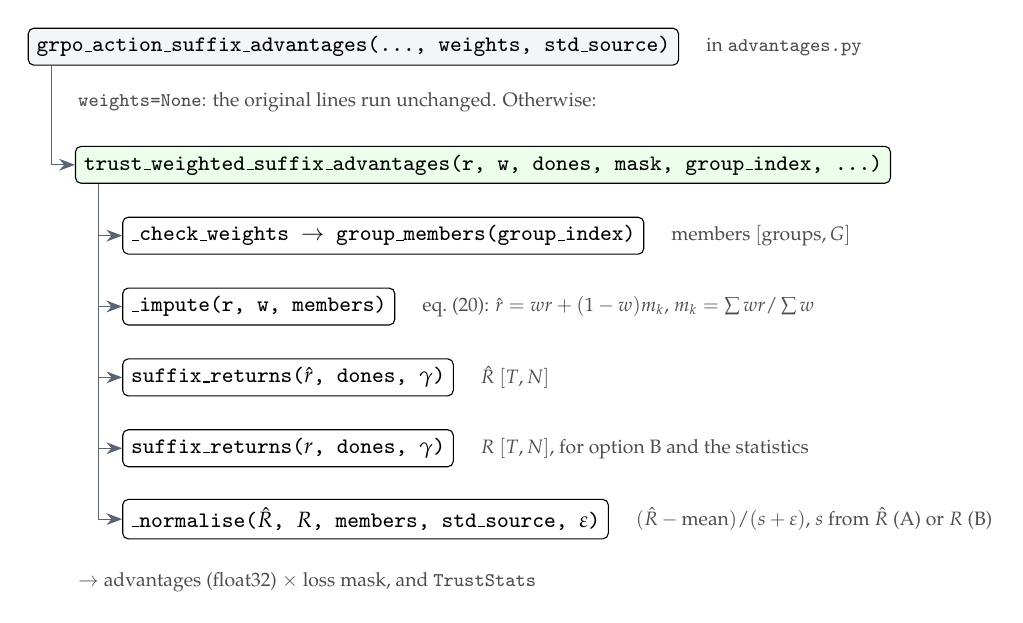
\begin{tikzpicture}[>={Stealth[length=2mm]},
  fn/.style={draw,rounded corners=2pt,font=\footnotesize\ttfamily,inner sep=3pt,anchor=west,fill=#1},
  fn/.default=white,
  dat/.style={font=\scriptsize,text=gray!60!black,anchor=west,align=left,inner sep=1pt},
  call/.style={->,draw=navy!70}]
\node[fn=blue!6] (g) at (0,0) {grpo\_action\_suffix\_advantages(..., weights, std\_source)};
\node[dat,right=3mm of g] {in \texttt{advantages.py}};
\node[dat] at (0.6,-0.7) {\texttt{weights=None}: the original lines run unchanged. Otherwise:};
\node[fn=green!8] (t) at (0.6,-1.5) {trust\_weighted\_suffix\_advantages(r, w, dones, mask, group\_index, ...)};
\node[fn] (cw) at (1.2,-2.4) {\_check\_weights $\to$ group\_members(group\_index)};
\node[dat,right=3mm of cw] {members $[\text{groups},G]$};
\node[fn] (im) at (1.2,-3.3) {\_impute(r, w, members)};
\node[dat,right=3mm of im] {eq.~(20): $\hat r=wr+(1-w)m_k$, $m_k=\sum wr/\sum w$};
\node[fn] (s1) at (1.2,-4.2) {suffix\_returns($\hat r$, dones, $\gamma$)};
\node[dat,right=3mm of s1] {$\hat R$ $[T,N]$};
\node[fn] (s2) at (1.2,-5.1) {suffix\_returns($r$, dones, $\gamma$)};
\node[dat,right=3mm of s2] {$R$ $[T,N]$, for option B and the statistics};
\node[fn] (no) at (1.2,-6.0) {\_normalise($\hat R$, $R$, members, std\_source, $\varepsilon$)};
\node[dat,right=3mm of no] {$(\hat R-\text{mean})/(s+\varepsilon)$, $s$ from $\hat R$ (A) or $R$ (B)};
\node[dat] at (0.6,-6.8) {$\to$ advantages (float32) $\times$ loss mask, and \texttt{TrustStats}};
\draw[call] ([xshift=3mm]g.south west) |- (t.west);
\foreach \n in {cw,im,s1,s2,no}{ \draw[call] ([xshift=3mm]t.south west) |- (\n.west); }
\end{tikzpicture}
\caption{Call tree of the trust-weighted advantages. In production the plugin will call \code{trust\_weighted\_suffix\_advantages} directly, with the cross-rank group ids (WP 5.1).}
\label{fig:trustflow}
\end{figure}

Two implementation details explain the tests. \code{group\_members} gathers each group into a $[T,\text{groups},G]$ layout that is exactly the reshape the old function used, which is what makes the $w\equiv1$ result \emph{bit}-identical, not just close. And all members enter the mean and std whatever their loss mask, as in both existing functions; the mask only multiplies the output.

\subsection{The FK reference fixture}
\code{make\_twin\_fk\_reference.main()} calls \code{load\_eef\_pose\_adapter()} and the repo's \code{ur5\_joint\_actions\_to\_eef\_states} in float64 on 1000 random joint vectors (seed 0), and writes the inputs and outputs with metadata (source hash, commit) to \code{tests/fixtures/twin\_fk\_reference\_ur5.json}. \code{test\_twin\_fk.py} compares \code{robot.fk} with it; a staleness test regenerates the table when torch is available and fails if the repo function changed.

%=====================================================================
\section{Where the next work packages plug in}\label{sec:next}
%=====================================================================
The roadmap's next modules fit into the graph of \cref{fig:deps} at fixed places. Building them in this position keeps the layering (no cycles, heavy imports lazy).

\begin{figure}[h]
\centering
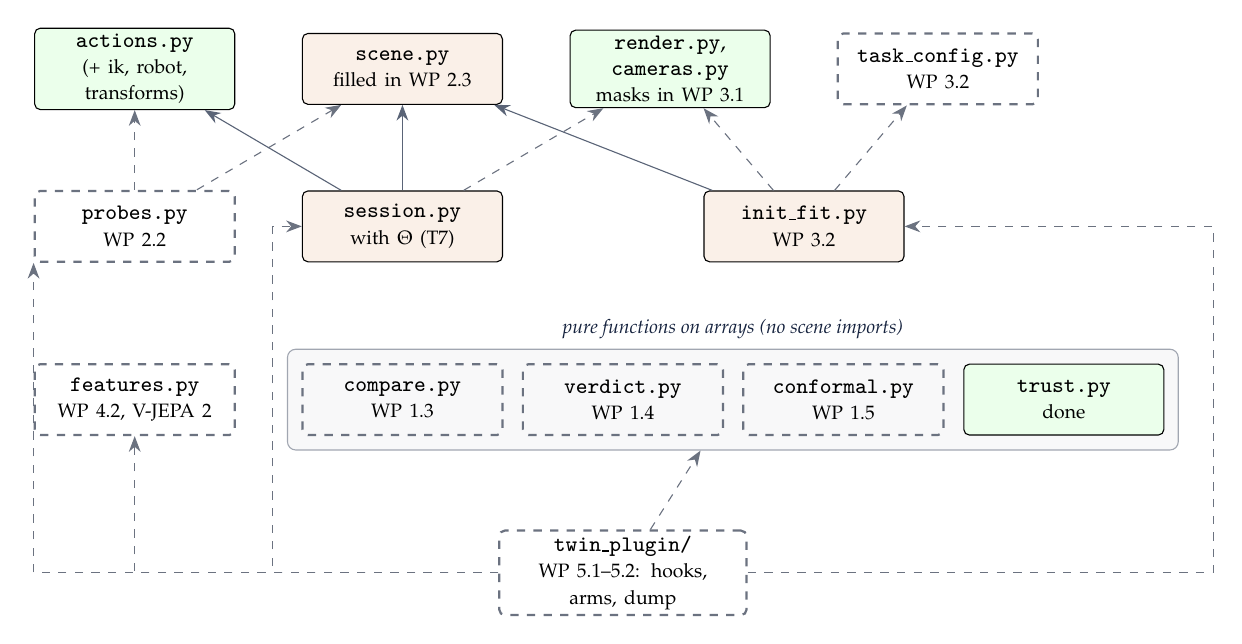
\begin{tikzpicture}[>={Stealth[length=2mm]},
  mod/.style={draw,rounded corners=2pt,font=\footnotesize,minimum height=9mm,text width=24mm,inner sep=2pt,align=center,fill=#1},
  mod/.default=white,
  new/.style={draw=plangray,dashed,thick,rounded corners=2pt,font=\footnotesize,minimum height=9mm,text width=24mm,inner sep=2pt,align=center},
  imp/.style={->,navy!70},
  nimp/.style={->,plangray,dashed}]
% existing, top row
\node[mod=green!8] (kin) at (0,0) {\texttt{actions.py}\\ \scriptsize (+ ik, robot, transforms)};
\node[mod=orange!10] (sc) at (3.4,0) {\texttt{scene.py}\\ \scriptsize filled in WP 2.3};
\node[mod=green!8] (rd) at (6.8,0) {\texttt{render.py}, \texttt{cameras.py}\\ \scriptsize masks in WP 3.1};
\node[new] (tc) at (10.2,0) {\texttt{task\_config.py}\\ \scriptsize WP 3.2};
% middle row
\node[new] (pr) at (0,-2.0) {\texttt{probes.py}\\ \scriptsize WP 2.2};
\node[mod=orange!10] (se) at (3.4,-2.0) {\texttt{session.py}\\ \scriptsize with $\Theta$ (T7)};
\node[mod=orange!10] (ifit) at (8.5,-2.0) {\texttt{init\_fit.py}\\ \scriptsize WP 3.2};
\draw[nimp] (pr) -- (kin); \draw[nimp] (pr) -- (sc);
\draw[imp] (se) -- (kin); \draw[imp] (se) -- (sc); \draw[nimp] (se) -- (rd);
\draw[imp] (ifit) -- (sc); \draw[nimp] (ifit) -- (rd); \draw[nimp] (ifit) -- (tc);
% pure functions group
\node[new] (ft) at (0,-4.2) {\texttt{features.py}\\ \scriptsize WP 4.2, V-JEPA 2};
\node[new] (cmp) at (3.4,-4.2) {\texttt{compare.py}\\ \scriptsize WP 1.3};
\node[new] (ver) at (6.2,-4.2) {\texttt{verdict.py}\\ \scriptsize WP 1.4};
\node[new] (con) at (9.0,-4.2) {\texttt{conformal.py}\\ \scriptsize WP 1.5};
\node[mod=green!8] (tw) at (11.8,-4.2) {\texttt{trust.py}\\ \scriptsize done};
\begin{scope}[on background layer]
\node[draw=navy!40,fill=navy!3,rounded corners=3pt,fit=(cmp)(ver)(con)(tw),inner sep=5pt,label={[font=\scriptsize\itshape,text=navy]above:pure functions on arrays (no scene imports)}] (pure) {};
\end{scope}
% plugin
\node[new,text width=30mm] (pl) at (6.2,-6.4) {\texttt{twin\_plugin/}\\ \scriptsize WP 5.1--5.2: hooks, arms, dump};
\draw[nimp] (pl.west) -- (1.75,-6.4) |- (se.west);
\draw[nimp] (pl.west) -| (ft);
\draw[nimp] (pl) -- (pure);
\draw[nimp] (pl.east) -- (13.7,-6.4) |- (ifit.east);
\draw[nimp] (pl.west) -| (pr.south west);
\end{tikzpicture}
\caption{Where the planned modules (dashed) sit, and what they will import. The Phase-1 modules are pure functions on arrays and import nothing from the scene; only the plugin ties the pieces together.}
\label{fig:next}
\end{figure}

\begin{center}\small
\begin{tabularx}{\linewidth}{@{}>{\raggedright\arraybackslash}p{3.4cm}>{\raggedright\arraybackslash}p{2.0cm}X@{}}
\toprule
\textbf{Module} & \textbf{WP} & \textbf{Proposal step and role}\\
\midrule
\code{compare.py} & 1.3 & Step 4: change features, $\tilde D$, grounded scores $S$ and spread $\kappa$ (on feature arrays)\\
\code{verdict.py} & 1.4 & Step 6.3--6.4: twin decision, Ctrl-World significance, verdict table, $p_{i,0}$\\
\code{conformal.py} & 1.5 & Step 7: conformal threshold, divergence chunk, $g_{i,k}$; Step 5 calibration rules\\
\code{probes.py} & 2.2 & Step 6.2: probe generator and null action, feasibility through \code{ActionsToJoints}\\
\code{scene.py (filled)} & 2.3 & Step 1, 3: laptop physics (T3)\\
\code{cameras.py, render.py (masks)} & 3.1 & Step 1, 3: MJCF cameras, segmentation masks (T4)\\
\code{task\_config.py, init\_fit.py} & 3.2 & Step 2: per-task configuration, render-and-compare fit (T5)\\
\code{features.py} & 4.2 & Step 4: V-JEPA 2 window features $\phi_t$\\
\code{twin\_plugin/} & 5.1--5.2 & integration hooks, arm modes, rollout dump \wt{8}\\
\bottomrule
\end{tabularx}
\end{center}

\appendix
%=====================================================================
\section{Data types passed between modules}
%=====================================================================
\begin{center}\small
\begin{tabularx}{\linewidth}{@{}>{\raggedright\arraybackslash}p{3.0cm}>{\raggedright\arraybackslash}p{2.4cm}X@{}}
\toprule
\textbf{Type} & \textbf{Defined in} & \textbf{Fields (shapes for one chunk)}\\
\midrule
\code{ActionReport} & actions & \code{ok}, \code{errors}, \code{warnings}, plus per-step diagnostics (step sizes, rot6d residuals, flags)\\
\code{EEFTargets} & actions & \code{policy\_states} $(B,32,7)$, \code{ctrl\_states} $(B,64,7)$, \code{ctrl\_condition} $(B,64,7)$, \code{next\_state} $(B,7)$\\
\code{IKResult} & ik & \code{q} $(6,)$, \code{converged}, \code{iters}, \code{pos\_err}, \code{rot\_err}, \code{at\_limit} $(6,)$, \code{min\_singular\_value}\\
\code{PathIKResult} & ik & \code{q} $(64,6)$, \code{converged} $(64,)$, \code{pos\_err}, \code{rot\_err}, \code{at\_limit} $(64,6)$, \code{joint\_step}, \code{speed\_violation}, \code{min\_singular\_value}, \code{branch\_switch}, \code{iters}; \code{feasible}\\
\code{JointChunk} & actions & \code{q} $(64,6)$, \code{gripper} $(64,)$, \code{eef}, \code{action\_check}, \code{ik}, \code{next\_state} $(7,)$; \code{feasible}\\
\code{SceneState} & scene & \code{laptop\_xy} $(2,)$, \code{laptop\_yaw}, \code{lid\_angle} (0 = closed), \code{q} $(6,)$, \code{gripper}\\
\code{ChunkRollout} & scene & \code{states} (list), \code{lid\_angle}, \code{contact\_finger\_lid}, \code{max\_penetration} (64 values each)\\
\code{ChunkResult} & session & \code{joints}, \code{rollout}, \code{renders} (dict per camera)\\
\code{EpisodeFit} & init\_fit & \code{episode\_id}, \code{best}, \code{near\_optimal}, \code{iou\_per\_view}, \code{q0}\\
\code{TrustStats} & trust & \code{weight\_below\_one\_share}, \code{weight\_mean}, \code{std\_ratio} $[T,\text{groups}]$, \code{adv\_abs\_max}\\
\bottomrule
\end{tabularx}
\end{center}

\end{document}
